\section{Solution}
\label{sec:solution}

\subsection{Cluster Analysis Results Visualization}

As was discussed before in the Section~\ref{dataset_description} cluster analysis result graph is binary tree.

"A binary tree is a connected acyclic graph such that the degree of each vertex is no more than 3. A rooted binary tree is such a graph that has one of its vertices of degree no more than 2 singled out as the root. With the root thus chosen, each vertex will have a uniquely defined parent, and up to two children; however, so far there is insufficient information to distinguish a left or right child. If we drop the connectedness requirement, allowing multiple connected component in the graph, we call such a structure a forest"~\cite{BINARY_TREE} Simple binary tree showed on the Figure~\ref{simple_binary_tree}

\begin{figure}[h!]
\centering
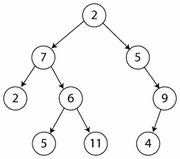
\includegraphics[scale=1.0]{pictures/simple_binary_tree.png}
\caption{A simple binary tree graph}
\label{simple_binary_tree}
\end{figure}

There several visualization methods for binary trees and more specific methods for cluster result. The main method for visualizing clusters is - dendrogram. Here is sample dendrogram visualization on the Figure~\ref{dendrogram_1} produced by MATLAB 7.2.

\begin{figure}[h!]
\centering
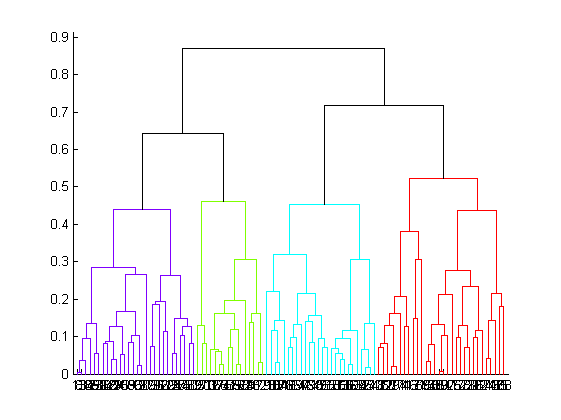
\includegraphics[scale=1.0]{pictures/dendrogram.png}
\caption{Dendrogram}
\label{dendrogram_1}
\end{figure}


The Figure~\cite{polardendrogram} shows polar dendrogram visualization algorithm of the same cluster tree produced by MATLAB.

\begin{figure}[h!]
\centering
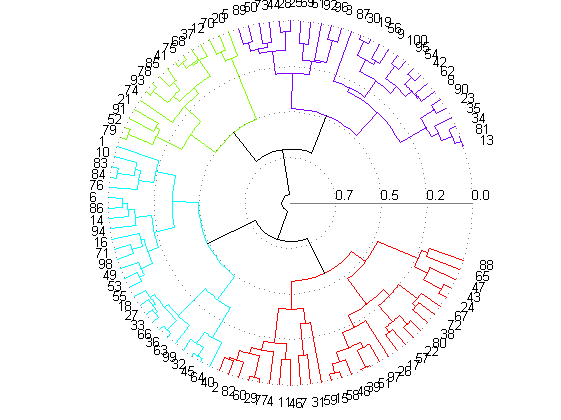
\includegraphics[scale=1.0]{pictures/polardendrogram.png}
\caption{Polar Dendrogram}
\label{polardendrogram}
\end{figure}

One of the main ideas was to use polar dendrogram algorithm for cluster visualization. The Figure~\cite{JUNG_radial_layout} shows visualization of the Cluster using native JUNG radial layout algorithm. Red are nodes and white is edges, black is background. As picture shows algorithm doesn't count nature of the cluster - very deep binary tree not wide as it is common for cluster analysis results, that's why it has many edge everlappings.


\begin{figure}[h!]
\centering
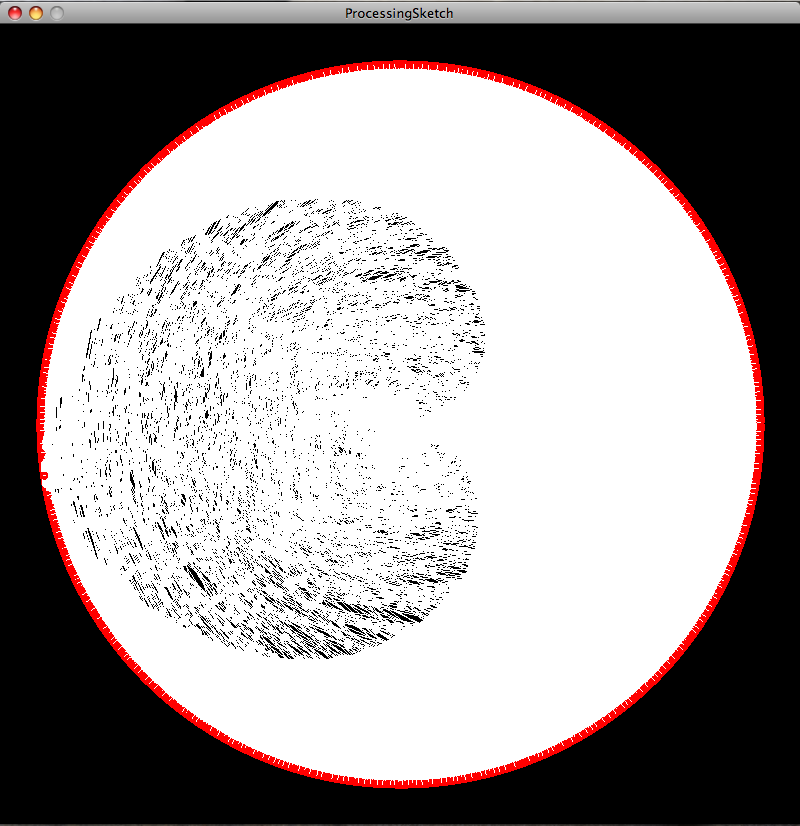
\includegraphics[scale=0.3]{pictures/using_JUNG_radial.png}
\caption{Cluster visualization using JUNG radial layout}
\label{JUNG_radial_layout}
\end{figure}


Also to visualization issue it has performance issue -- without any measurement was seen for an eye that program does not allow smooth interaction. Low performance issue was in nature of the visualization in the JUNG: it uses very complex hierarchical structure with many utility classes per visualized object and the cost is big memory usage. Also JUNG uses Java 2D~\cite{JAVA_2D} which by itself is "heavyweight" because it's part of the Java AWT -- Abstract Windows Toolkit.


"The Abstract Window Toolkit (AWT) is Java's original platform-independent windowing, graphics, and user-interface widget toolkit. The AWT is now part of the Java Foundation Classes (JFC) � the standard API for providing a graphical user interface (GUI) for a Java program. When Sun Microsystems first released Java in 1995, AWT widgets provided a thin level of abstraction over the underlying native user interface. For example, creating an AWT check box would cause AWT directly to call the underlying native subroutine that created a check box."~\cite{JAVA_AWT} This technology is outdated and replaced by Swing.


"Swing is the primary Java GUI widget toolkit. It is part of Sun Microsystems' Java Foundation Classes (JFC) � an API for providing a graphical user interface (GUI) for Java programs.
Swing was developed to provide a more sophisticated set of GUI components than the earlier Abstract Window Toolkit. Swing provides a native look and feel that emulates the look and feel of several platforms, and also supports a pluggable look and feel that allows applications to have a look and feel unrelated to the underlying platform."~\cite{JAVA_SWING}


"Since early versions of Java, a portion of the Abstract Window Toolkit (AWT) has provided platform-independent APIs for user interface components. In AWT, each component is rendered and controlled by a native peer component specific to the underlying windowing system.
By contrast, Swing components are often described as lightweight because they do not require allocation of native resources in the operating system's windowing toolkit. The AWT components are referred to as heavyweight components."~\cite{JAVA_SWING} More detail comparison can be found here.~\cite{AWT_VS_SWING}


The Figure~\ref{cluster_jogl_impl} shows improved JUNG radial algorithm and own visualization implementation using JOGL. JOGL will be discussed in the Section~\ref{opengl}.


\begin{figure}[h!]
\centering
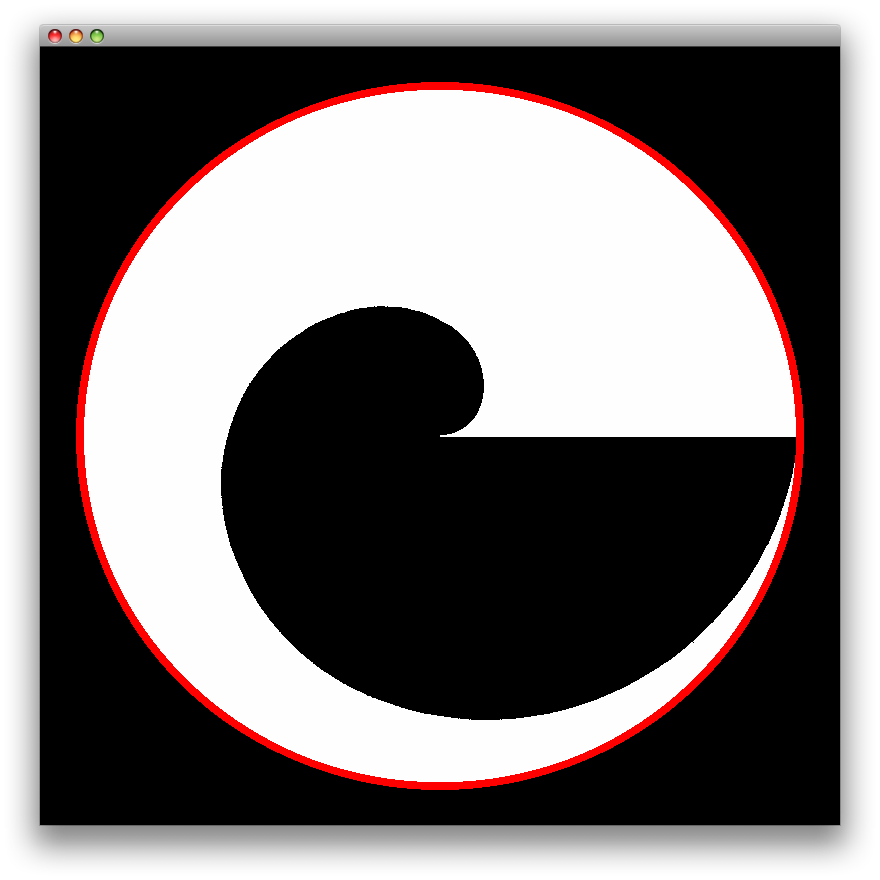
\includegraphics[scale=0.3]{pictures/cluster_jogl_impl.png}
\caption{Cluster visualization using JOGL and improved JUNG radial layout}
\label{cluster_jogl_impl}
\end{figure}


The Figure~\ref{cluster_jogl_impl_with_subgraph_1} and Figure~\ref{cluster_jogl_impl_with_subgraph_2} shows cluster visualization and highlighted subgraph using algorithm that was discussed in the Section~\ref{problem_statement_and_goal}. This pictures show the nature of the dataset. Improved version has good performance and better visualization but still has issues. Too many elements are in the scene, it is impossible to identify separate gene and trace highlighted graph genes.

\begin{figure}[h!]
\centering
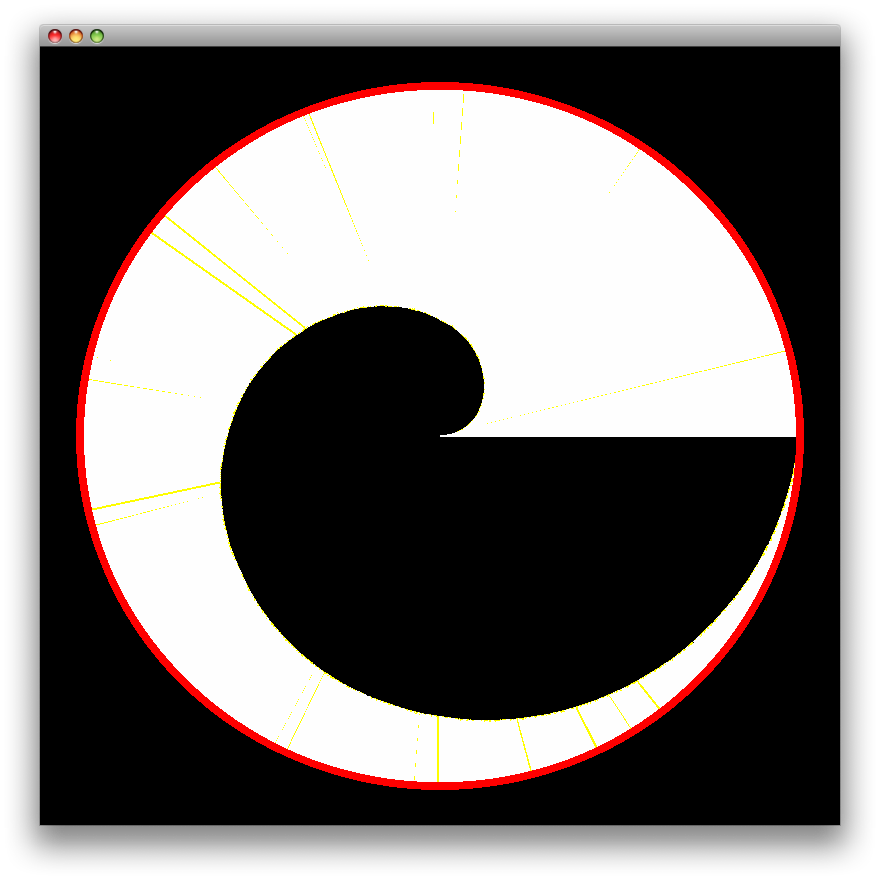
\includegraphics[scale=0.3]{pictures/cluster_jogl_impl_with_subgraph_1.png}
\caption{Cluster graph and highlighted subgraph}
\label{cluster_jogl_impl_with_subgraph_1}
\end{figure}

\begin{figure}[h!]
\centering
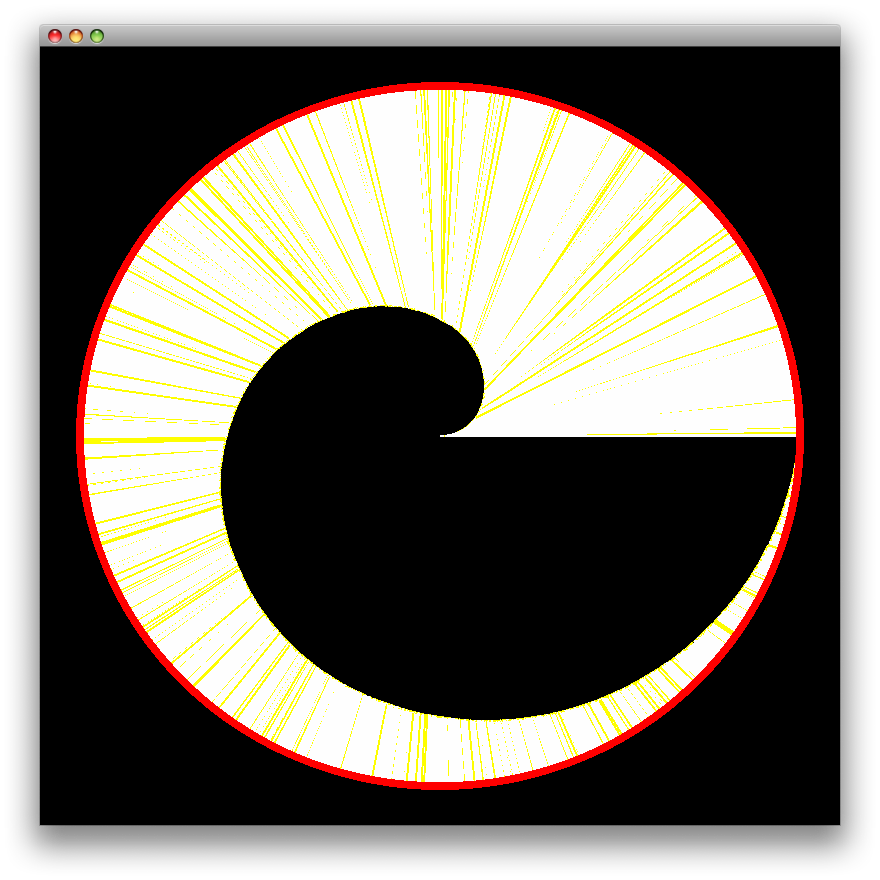
\includegraphics[scale=0.3]{pictures/cluster_jogl_impl_with_subgraph_2.png}
\caption{Cluster graph and highlighted subgraph}
\label{cluster_jogl_impl_with_subgraph_2}
\end{figure}


\subsection{Gene Ontology Visualization}
